
\section{Organizing DMA Risks}\label{sec:dma-risks}
%In this section we organize and categorize the risks associated with DMA operations.
%We first categorise the different types of \subpage{} vulnerabilities.
%Then, we categorize the three vulnerability attributes, providing building blocks for reasoning about code-injection attacks.\adam{similar comment to intro: not clear what this trifecta means on top of the first categorization}
%These paint a clear picture of risks and dangers posed by DMA capable devices.
%We also discuss dangerous trade-offs and discuss the threat model.
%\adam{similar comment to intro: not clear what this trifecta means on top of the first categorization}
This section organizes and categorizes the risks associated with DMA operations, providing the building blocks for reasoning about code injection attacks.
\DIFdelbegin \DIFdel{In particular, we }\DIFdelend \DIFaddbegin \DIFadd{We }\DIFaddend first present our threat model \DIFdelbegin \DIFdel{. Then, we categorise }\DIFdelend \DIFaddbegin \DIFadd{and then organize }\DIFaddend the different \subpage{} vulnerabilities into four categories.
Finally, we identify a set of three vulnerability attributes that make it possible for a malicious device to exploit a \subpage{} vulnerability and execute a viable code injection attack.

\subsection{Threat Model}\label{sec:threat_model}
\DIFdelbegin \DIFdel{Our organization of DMA risksin this section reveals }\DIFdelend \DIFaddbegin \DIFadd{By organizing the DMA risks, we reveal }\DIFaddend that the Linux kernel is vulnerable to various high impact attacks.
For example, a full memory dump is possible when an attacker can modify data pointers before they are mapped, causing the driver to map arbitrary kernel addresses.
Alternatively, a malicious device can corrupt random memory regions~\cite{MMT16}\DIFaddbegin \DIFadd{, }\DIFaddend resulting in a denial of service attack (DOS).


\DIFdelbegin \DIFdel{Nevertheless, the }\DIFdelend \DIFaddbegin \DIFadd{The }\DIFaddend most significant potential consequence of \DIFdelbegin \DIFdel{our }\DIFdelend \DIFaddbegin \DIFadd{these }\DIFaddend attacks is privilege escalation via code injection, allowing attackers to execute arbitrary code with kernel privileges. Indeed, this is the focus of our paper. 
Our attacks are designed with the following assumptions:
\begin{enumerate}
    \item \DIFdelbegin \DIFdel{We assume the existence of a }\DIFdelend \DIFaddbegin \DIFadd{A }\DIFaddend malicious DMA-capable device \DIFaddbegin \DIFadd{is }\DIFaddend attached to the system.
    \item The actual attack is performed solely by the DMA-capable malicious device.
    \item Any hardware aside from the specific malicious device is working as expected.
 \end{enumerate}


%However other high impact attacks may still be viable with only part of the vulnerability attributes. 
%For example, a full memory dump. 

%\textcolor{green}{In this scenario, an attacker is able to modify the kernel control flow in such a way as to cause it to map arbitrary kernel addresses. Given write access to an I/O scatter-gather list, a malicious device can control which memory pages are mapped by the CPU to the device.}



%This would result in a full memory dump or a random memory corruption, resulting in a denial of service~\cite{MMT16}. 

%\adam{this subsection is very short and hard to follow, why is it needed? suggest expanding or deleting}

%
%
%Another potential consequences of our findings one may consider is a full system memory dump
%. These are harder to thwart and even harder to detect. Lastly, a consequence of a possible failed attack is 
%or a random memory corruption, resulting in a denial of service~\cite{MMT16}. 
%Clearly, malformed devices should not be able to crash the entire system. 
%
%
%
%
% \subsection{\textcolor{red}{Other attacks - Integrate?}}
% \textcolor{green}{Move to Threat model and Fix}
% The focus of our work is on code injection attacks as they often have a much higher value for the attacker (e.g., get access to sensitive machines and data). 
% However other high impact attacks may still be viable with only part of the vulnerability attributes. 
% For example, a full memory dump.
% %The MMO schema can be extended  for additional vulnerability analysis. For example, other high impact attacks, such as a full memory dump, may still be viable with only \means and \oportunity{} given.
% %KASLR is designed to stop code injection attacks. This indeed holds as long as kernel pointers are not leaked, an assumption that is not valid for DMA capable devices. For example, an OS leaks kernel pointers to a NIC, on pages containing small TX buffers. A malicious NIC can even spoof seemingly legitimate packets (e.g., ARP, ICMP, ICMPv6) to trigger kernel pointer leakage.
% %Both attack types use type (d) vulnerability to compromise KASLR. KASLR is designed to stop code injection attacks. This indeed holds as long as kernel pointers are not leaked, an assumption that is not valid for DMA capable devices. For example, an OS leaks kernel pointers to a NIC, on pages containing small TX buffers. A malicious NIC can even spoof seemingly legitimate packets (e.g., ARP, ICMP, ICMPv6) to trigger kernel pointer leakage. \textcolor{olive}{We demonstrate the risks associated with type (d) vulnerability in Sec.~\ref{fig:dkasan-report}.}
% In this scenario, an attacker is able to modify the kernel control flow in such a way as to cause it to map arbitrary kernel addresses. Given write access to an I/O scatter-gather list, a malicious device can control which memory pages are mapped by the CPU to the device. This would result in a full memory dump.\adam{this subsection is very short and hard to follow, why is it needed? suggest expanding or deleting}
%\adam{description isn't clear: it's modifying control-flow, so is it a code injection attack?} 
%In order to achieve this, an attacker needs to modify a kernel pointer once before it is mapped and, for a second time before send (i.e., TX) completion in order to avoid memory corruption (Sec.~\ref{sec:linux_net}). 

%We demonstrate in Section~\ref{sec:linux_net}, how an adversary can take advantage of \emph{deferred} mode.



\subsection{Sub-Page Vulnerabilities}\label{sec:subpage}

%\adam{start with a sentence defining what a subpage vuln is (IO buffer co-located with data)}
Anytime an I/O buffer smaller than a page is DMA-mapped\DIFaddbegin \DIFadd{, }\DIFaddend all additional information that resides on the same physical page becomes accessible to the device. Any such situation where a memory-region is exposed due to the IOMMU page granularity is called a \subpage vulnerability.

We classify the different types of \subpage \DIFdelbegin \DIFdel{vulnerability }\DIFdelend \DIFaddbegin \DIFadd{vulnerabilities }\DIFaddend into four categories\DIFaddbegin \DIFadd{, }\DIFaddend as illustrated in \DIFdelbegin \DIFdel{Fig.}\DIFdelend \DIFaddbegin \DIFadd{Figure}\DIFaddend ~\ref{fig:colocation}:

\begin{enumerate}
    \item[(a)] The I/O buffer is part of a bigger data structure. This data structure may include function pointers, often caused by poor DMA hygiene \DIFdelbegin \DIFdel{by }\DIFdelend \DIFaddbegin \DIFadd{in }\DIFaddend the driver. An isolated driver fix is usually sufficient to \DIFdelbegin \DIFdel{fix }\DIFdelend \DIFaddbegin \DIFadd{repair }\DIFaddend such vulnerabilities.
    \item[(b)] The OS (e.g., memory allocator)---rather than the driver---saves metadata \DIFdelbegin \DIFdel{, }\DIFdelend such as free-lists, on the same page as the I/O buffer~\cite{Cor07}. Manipulating these data structures may also compromise the system~\cite{ak09}. \DIFdelbegin \DIFdel{Similarly }\DIFdelend \DIFaddbegin \DIFadd{Similar }\DIFaddend to (a), sensitive metadata is unwittingly shared. However, in this case, it is an OS subsystem that is at fault rather than the device driver.
    \item[(c)] The same page is mapped multiple times due to co-located device driver buffers\DIFaddbegin \DIFadd{, }\DIFaddend resulting in multiple \iova{}\DIFaddbegin \DIFadd{s }\DIFaddend indicating the same page. 
    In this case, unmapping one \iova will not \DIFdelbegin \DIFdel{stop }\DIFdelend \DIFaddbegin \DIFadd{prevent }\DIFaddend the device from accessing the page through a different \iova.
    The device will retain access to the physical page as long as a single valid \iova{} exists. This means that the device can tamper with memory regions that should no longer be accessible\DIFdelbegin \DIFdel{to it}\DIFdelend . We discuss the practical implications of multiple \iova indicating the same page in \DIFdelbegin \DIFdel{Sec.}\DIFdelend \DIFaddbegin \DIFadd{Section}\DIFaddend ~\ref{sec:timely}.
    \item[(d)] The I/O buffer and a different, dynamically allocated memory buffer may coincidentally share a page. This common situation results in data leakage (e.g., kernel pointers). Currently, the Linux kernel uses the same \DIFaddbegin \DIFadd{kmalloc }\DIFaddend memory allocation mechanism \DIFdelbegin \DIFdel{(e.g., kmalloc) }\DIFdelend for both I/O buffers and regular kernel buffers. Consequently, I/O buffers often share pages with other, potentially sensitive, kernel buffers. Since IOMMU works \DIFdelbegin \DIFdel{in }\DIFdelend \DIFaddbegin \DIFadd{at }\DIFaddend page granularity, the respective I/O devices gain access to these kernel buffers. Such vulnerability is a subclass of (b), as \DIFaddbegin \DIFadd{it is caused by }\DIFaddend an OS subsystem\DIFdelbegin \DIFdel{causes it, but }\DIFdelend \DIFaddbegin \DIFadd{; }\DIFaddend the main difference is that the exposed data structures are leaked randomly.
\end{enumerate}
%\adam{what does point (c) have to do with sub-page vulns? It seems generic, and indeed, it doesn't talk about any co-location.}\SV{Type C is key to gaining opportunity in \compound attacks, we've fixed the first paragraph to fit better.}

\begin{figure}[t]
    \centering
    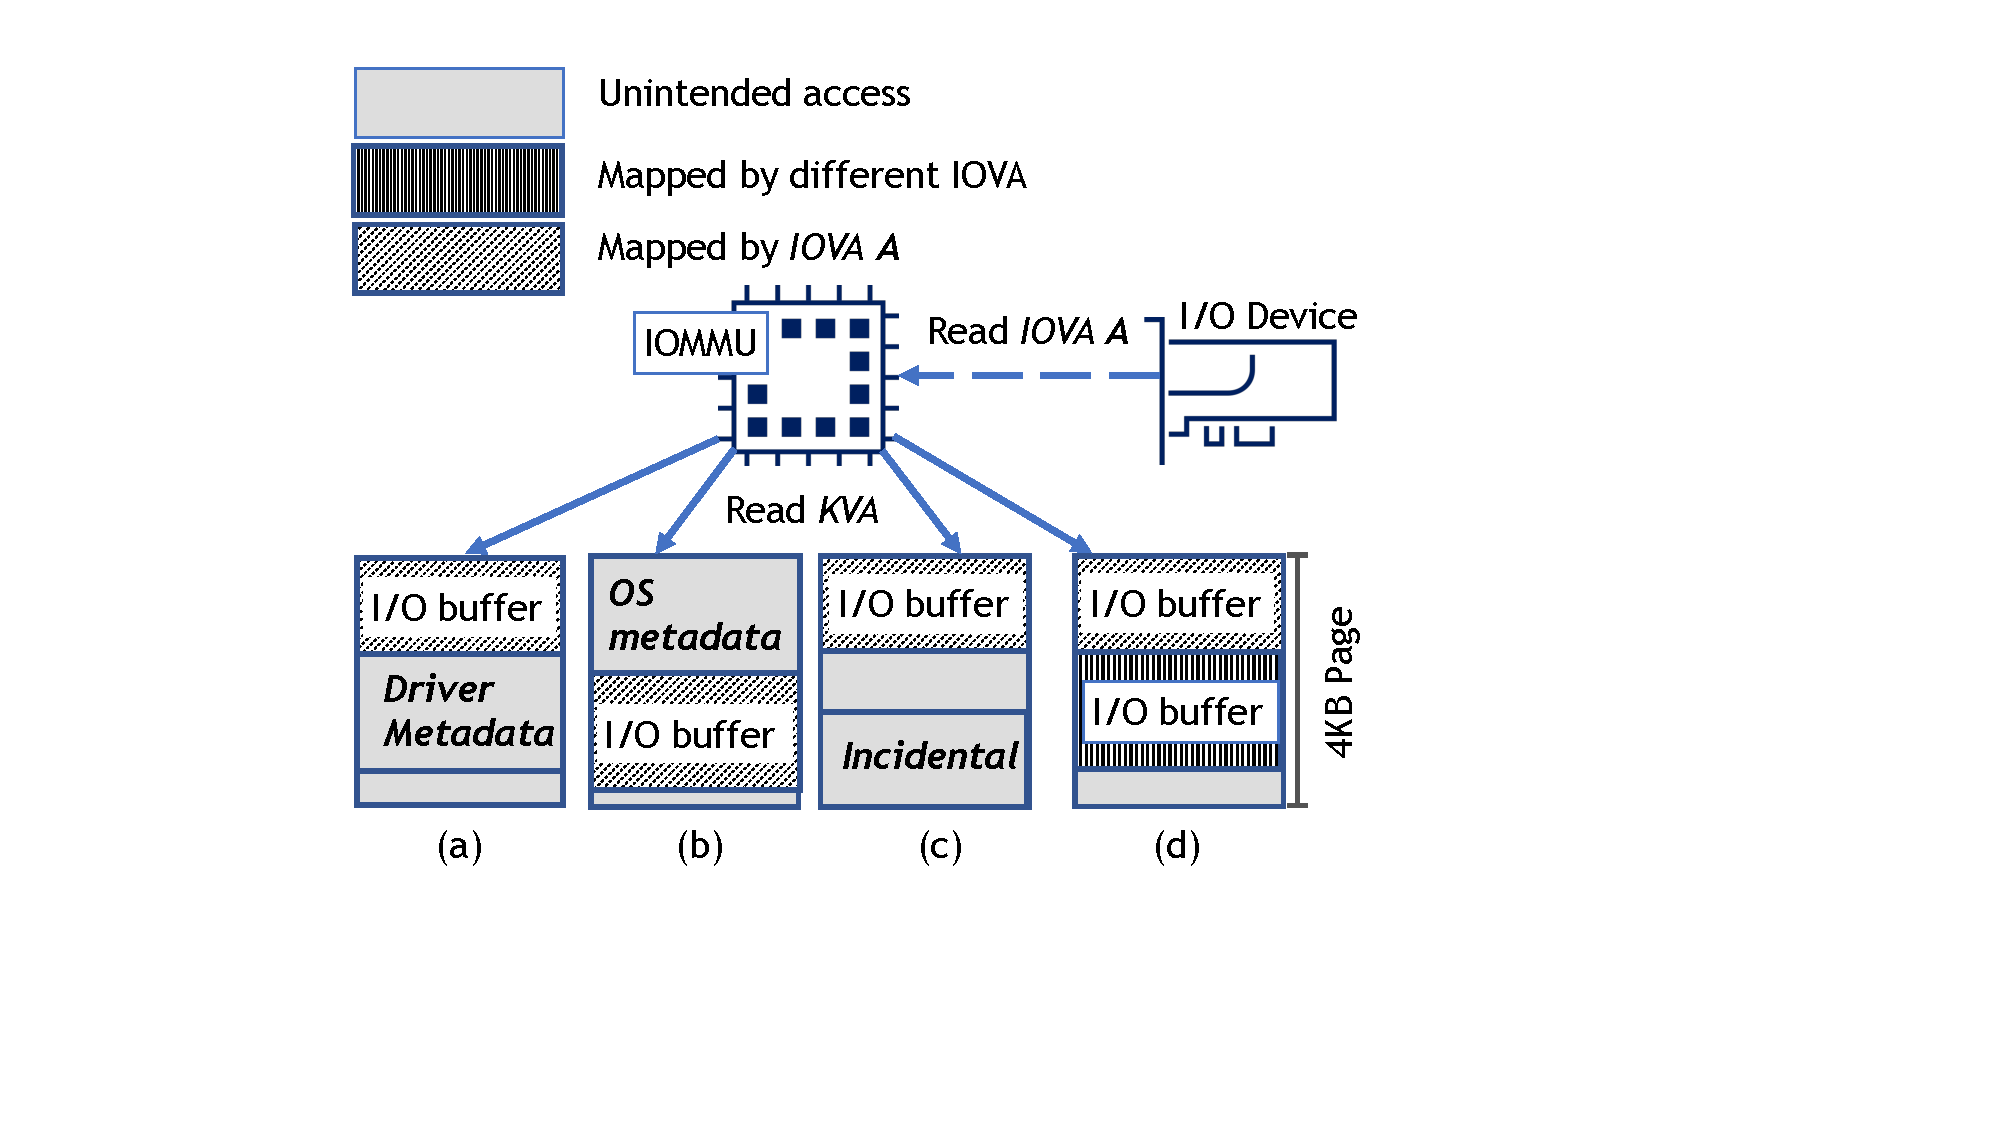
\includegraphics[width=0.8\columnwidth]{figs/subpage.pdf}
    \caption{\DIFdelbeginFL %DIFDELCMD < \subpage{} %%%
\DIFdelendFL DMA \DIFaddbeginFL \subpage{} \DIFaddendFL vulnerabilities when the I/O buffer shares a page with other data: (a) I/O buffer metadata; (b) OS
metadata; (c) a page mapped by multiple \iova; (d) randomly co-located sensitive buffers.}
%\vspace{-3mm}
    \label{fig:colocation}
\end{figure}


%In the next sections we demonstrate how a \simple{} attack utilizes type (a) vulnerability (Sec.~\ref{sec:sbp2_attack}). A \emph{compound attack}, on the other hand, uses type (b) and (c) vulnerabilities (Sec.~\ref{sec:linux_net}). 
%We also demonstrate the risks associated with type (d) vulnerability in Sec.~\ref{sec:dma-kasan}. Type (d) vulnerability simplifies KASLR subversion~(\ref{sec:kaslr}) and opens viable attack vectors. 


\subsection{Vulnerability Attributes for Code Injection}\label{sec:mmo}

We introduce a schema that allows for a systematic analysis of code injection attacks by DMA-capable devices.
%to categorizes DMA vulnerabilities. The goal of MMO is to define building blocks for reasoning about DMA attacks.
For a successful privilege escalation attack (i.e., code injection), a malicious device needs the following set of three vulnerability attributes:
\begin{enumerate}
    \item The \kva{} of a kernel buffer filled with malicious code (e.g., \DIFdelbegin \DIFdel{a }\DIFdelend ROP attack). Given \DIFaddbegin \DIFadd{that }\DIFaddend the device is using an \iova, the attacker needs to obtain the buffer's \kva{}, for example, by observing leaked pointers. 
    \item Write access to a function callback pointer, which can alter the CPU control flow and cause it to execute the malicious code. For example, \DIFaddbegin \DIFadd{this might be }\DIFaddend write access to a data structure that holds a function callback pointer at a known offset.\footnote{The Linux kernel randomizes the layout of some data structures with \_\_randomize\_layout annotation~\cite{rand_layout}.} The location on the page of the callback pointer must be known to the device.
    %\item There exists a time window such that modifying the function pointer during that time window is followed by the CPU reading the pointer without previously altering its content.
    \item A time window exists such that the device can modify the callback pointer during that window and the CPU will subsequently jump to the pointed code\DIFdelbegin \DIFdel{(}\DIFdelend \DIFaddbegin \DIFadd{; this occurs }\DIFaddend before the pointer gets overwritten, if it is ever overwritten\DIFdelbegin \DIFdel{)}\DIFdelend .
\end{enumerate}

To further emphasize the significance of these attributes, we present a hypothetical scenario. Assume a NIC has write access to a page containing a received (RX) packet. Due to a \subpage{} vulnerability and a random allocation coincidence (\DIFdelbegin \DIFdel{Fig.}\DIFdelend \DIFaddbegin \DIFadd{Figure}\DIFaddend ~\ref{fig:colocation}, type (d)), a structure with a callback pointer is write-accessible to a malicious device. Also, the device can create a valid \mabaf{} in the aforementioned page. It may seem that the device has a valid attack, whereas it actually lacks the following:

\begin{itemize}
    \item Without a valid \kva{} of the writable page, the device cannot modify the callback function pointer to indicate the \mabaf.
    \item Although a callback function pointer is available for modifications, the device has no way of knowing: 
    \begin{enumerate}
        \item[(a)] That a callback function pointer is available for sabotage.
        \item[(b)] The correct offset of the callback function pointer.
    \end{enumerate}
    \item It is not known \DIFdelbegin \DIFdel{if }\DIFdelend \DIFaddbegin \DIFadd{whether }\DIFaddend the modified callback pointer will be executed.
\end{itemize}

Under the hypothesized circumstance, and without additional information, a malicious device has no viable attack options.
\DIFdelbegin \DIFdel{Namely, all }\DIFdelend \DIFaddbegin \DIFadd{All }\DIFaddend three attributes are required for a code injection attack.
While corrupting \DIFaddbegin \DIFadd{the }\DIFaddend random kernel memory is still a possibility and may even cause a kernel panic~\cite{MMT16}, it does not achieve the goal of privilege escalation.
